% PARTE 3/3: EJERCICIOS PROPUESTOS Y SOLUCIONES DETALLADAS
% Tema: Transformaciones de funciones trigonométricas
% Grado 10

\section{Ejercicios Propuestos}

Ahora es tu turno. Resuelve los siguientes ejercicios aplicando lo que has aprendido sobre transformaciones de funciones trigonométricas. Las soluciones detalladas están en la siguiente sección, pero intenta resolverlos primero por tu cuenta. ¡Dale con todo!

\begin{ejercicio}[title=Ejercicio 1]
Dada la función $f(x) = 3\sin(x)$, identifica todas las transformaciones aplicadas a la función básica $y = \sin(x)$ y determina:
\begin{itemize}
    \item[a)] La amplitud de la función
    \item[b)] El período de la función
    \item[c)] El rango de la función
    \item[d)] Los valores máximo y mínimo
\end{itemize}
\end{ejercicio}

\begin{ejercicio}[title=Ejercicio 2]
Para la función $g(x) = \cos(2x)$, determina:
\begin{itemize}
    \item[a)] El período de la función
    \item[b)] El número de ciclos completos en el intervalo $[0, 2\pi]$
    \item[c)] Las coordenadas de los puntos donde la función alcanza su valor máximo en $[0, 2\pi]$
\end{itemize}
\end{ejercicio}

\begin{ejercicio}[title=Ejercicio 3]
Analiza la función $h(x) = \sin(x - \frac{\pi}{4})$ y determina:
\begin{itemize}
    \item[a)] El tipo de desfase (horizontal) aplicado
    \item[b)] La dirección del desfase (izquierda o derecha)
    \item[c)] El valor de $h(0)$
    \item[d)] El primer valor positivo de $x$ donde $h(x) = 1$
\end{itemize}
\end{ejercicio}

\begin{ejercicio}[title=Ejercicio 4]
Dada la función $k(x) = -2\cos(x) + 1$, identifica:
\begin{itemize}
    \item[a)] Todas las transformaciones aplicadas a $y = \cos(x)$
    \item[b)] La amplitud
    \item[c)] El valor máximo y mínimo de la función
    \item[d)] El eje de simetría (línea central)
\end{itemize}
\end{ejercicio}

\begin{ejercicio}[title=Ejercicio 5]
Grafica la función $f(x) = 2\sin(3x)$ en el intervalo $[0, 2\pi]$ y determina:
\begin{itemize}
    \item[a)] La amplitud
    \item[b)] El período
    \item[c)] El número de ciclos completos en $[0, 2\pi]$
    \item[d)] Las coordenadas de los primeros tres máximos
\end{itemize}
\end{ejercicio}

\begin{ejercicio}[title=Ejercicio 6]
Para la función $m(x) = \cos(x + \frac{\pi}{3}) - 2$, determina:
\begin{itemize}
    \item[a)] El desfase horizontal y su dirección
    \item[b)] El desfase vertical y su dirección
    \item[c)] El rango de la función
    \item[d)] Grafica la función en el intervalo $[-\pi, 2\pi]$
\end{itemize}
\end{ejercicio}

\begin{ejercicio}[title=Ejercicio 7]
Analiza la función $p(x) = 4\sin(\frac{1}{2}x - \pi) + 3$ y encuentra:
\begin{itemize}
    \item[a)] La amplitud
    \item[b)] El período
    \item[c)] El desfase horizontal (en función de la forma $\sin(B(x - C))$)
    \item[d)] El desfase vertical
    \item[e)] El rango de la función
\end{itemize}
\end{ejercicio}

\begin{ejercicio}[title=Ejercicio 8: Problema aplicado]
La altura de la marea en un puerto se puede modelar con la función:
\[
h(t) = 5\cos\left(\frac{\pi}{6}t\right) + 8
\]
donde $h$ está en metros y $t$ es el tiempo en horas después de la medianoche.
\begin{itemize}
    \item[a)] ¿Cuál es la altura máxima de la marea?
    \item[b)] ¿Cuál es la altura mínima de la marea?
    \item[c)] ¿Cuál es el período de la marea (tiempo entre dos mareas altas consecutivas)?
    \item[d)] ¿A qué hora ocurre la primera marea alta después de la medianoche?
    \item[e)] ¿Cuál es la altura de la marea a las 9:00 AM?
\end{itemize}
\end{ejercicio}

\newpage

\section{Soluciones Detalladas}

\begin{solucion}[title=Solucion Ejercicio 1]
\textbf{Dada:} $f(x) = 3\sin(x)$

\textbf{Análisis de transformaciones:}

La función básica es $y = \sin(x)$. La transformación aplicada es una multiplicación por 3, lo que representa un \textbf{estiramiento vertical} con factor 3.

\textbf{Parte a):} Amplitud

La amplitud es el valor absoluto del coeficiente que multiplica a la función seno:
\[
\text{Amplitud} = |3| = 3
\]

\textbf{Respuesta a):} $\boxed{\text{Amplitud} = 3}$

\textbf{Parte b):} Período

Como no hay transformaciones horizontales (el coeficiente de $x$ es 1), el período es el mismo que el de $\sin(x)$:
\[
\text{Período} = \frac{2\pi}{B} = \frac{2\pi}{1} = 2\pi
\]

\textbf{Respuesta b):} $\boxed{\text{Período} = 2\pi}$

\textbf{Parte c):} Rango

El rango de $\sin(x)$ es $[-1, 1]$. Al multiplicar por 3, el rango se estira:
\[
\text{Rango de } f(x) = [3(-1), 3(1)] = [-3, 3]
\]

\textbf{Respuesta c):} $\boxed{\text{Rango} = [-3, 3]}$

\textbf{Parte d):} Valores máximo y mínimo

Del rango, podemos ver que:
\begin{itemize}
    \item Valor máximo: $f_{\max} = 3$ (ocurre cuando $\sin(x) = 1$, es decir, en $x = \frac{\pi}{2} + 2\pi k$)
    \item Valor mínimo: $f_{\min} = -3$ (ocurre cuando $\sin(x) = -1$, es decir, en $x = \frac{3\pi}{2} + 2\pi k$)
\end{itemize}

\textbf{Respuesta d):} $\boxed{\text{Máximo} = 3, \quad \text{Mínimo} = -3}$

\textbf{Gráfica:}

\begin{center}
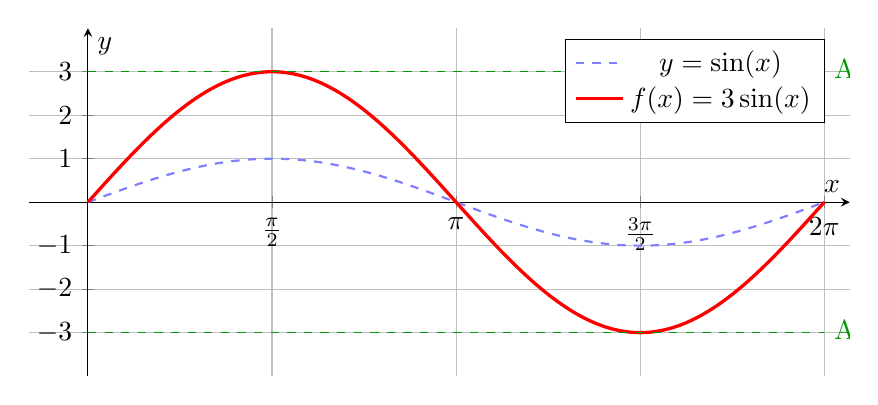
\begin{tikzpicture}
\begin{axis}[
    width=12cm,
    height=6cm,
    axis lines=middle,
    xlabel={$x$},
    ylabel={$y$},
    domain=0:2*pi,
    samples=200,
    ymin=-4,
    ymax=4,
    xmin=-0.5,
    xmax=6.5,
    xtick={0,1.5708,3.1416,4.7124,6.2832},
    xticklabels={$0$,$\frac{\pi}{2}$,$\pi$,$\frac{3\pi}{2}$,$2\pi$},
    ytick={-3,-2,-1,0,1,2,3},
    grid=major,
    legend pos=north east,
]
    % Función original
    \addplot[blue!50,dashed,thick] {sin(deg(x))};
    \addlegendentry{$y = \sin(x)$}

    % Función transformada
    \addplot[red,very thick] {3*sin(deg(x))};
    \addlegendentry{$f(x) = 3\sin(x)$}

    % Líneas de amplitud
    \draw[green!60!black,dashed] (axis cs:0,3) -- (axis cs:6.2832,3) node[right] {Amplitud = 3};
    \draw[green!60!black,dashed] (axis cs:0,-3) -- (axis cs:6.2832,-3) node[right] {Amplitud = 3};
\end{axis}
\end{tikzpicture}
\end{center}

\textbf{Verificación:}
\begin{itemize}
    \item En $x = \frac{\pi}{2}$: $f(\frac{\pi}{2}) = 3\sin(\frac{\pi}{2}) = 3(1) = 3$ \checkmark
    \item En $x = \frac{3\pi}{2}$: $f(\frac{3\pi}{2}) = 3\sin(\frac{3\pi}{2}) = 3(-1) = -3$ \checkmark
\end{itemize}
\end{solucion}

\begin{solucion}[title=Solucion Ejercicio 2]
\textbf{Dada:} $g(x) = \cos(2x)$

\textbf{Análisis:}

La transformación aplicada es un coeficiente $B = 2$ multiplicando a $x$, lo que representa una \textbf{compresión horizontal}.

\textbf{Parte a):} Período

El período se calcula con la fórmula:
\[
\text{Período} = \frac{2\pi}{B} = \frac{2\pi}{2} = \pi
\]

Esto significa que la función completa un ciclo completo en un intervalo de longitud $\pi$ (en lugar de $2\pi$ como la función básica).

\textbf{Respuesta a):} $\boxed{\text{Período} = \pi}$

\textbf{Parte b):} Número de ciclos en $[0, 2\pi]$

Si cada ciclo tiene longitud $\pi$, entonces en un intervalo de longitud $2\pi$ caben:
\[
\text{Número de ciclos} = \frac{2\pi}{\pi} = 2 \text{ ciclos completos}
\]

\textbf{Respuesta b):} $\boxed{2 \text{ ciclos completos}}$

\textbf{Parte c):} Puntos donde alcanza el valor máximo en $[0, 2\pi]$

La función coseno alcanza su valor máximo (que es 1) cuando el argumento es un múltiplo de $2\pi$:
\[
2x = 2\pi k, \quad k \in \mathbb{Z}
\]
\[
x = \pi k
\]

Para $x \in [0, 2\pi]$, los valores son:
\begin{itemize}
    \item $k = 0$: $x = 0$, $g(0) = \cos(0) = 1$ → Punto $(0, 1)$
    \item $k = 1$: $x = \pi$, $g(\pi) = \cos(2\pi) = 1$ → Punto $(\pi, 1)$
    \item $k = 2$: $x = 2\pi$, $g(2\pi) = \cos(4\pi) = 1$ → Punto $(2\pi, 1)$
\end{itemize}

\textbf{Respuesta c):} $\boxed{(0, 1), \quad (\pi, 1), \quad (2\pi, 1)}$

\textbf{Gráfica:}

\begin{center}
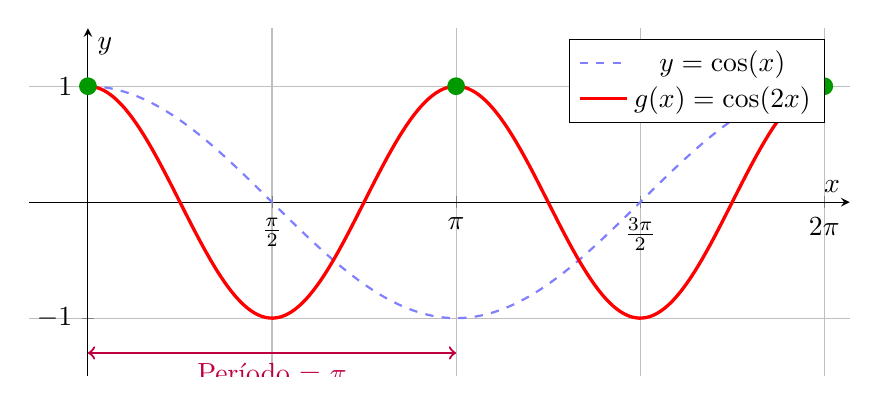
\begin{tikzpicture}
\begin{axis}[
    width=12cm,
    height=6cm,
    axis lines=middle,
    xlabel={$x$},
    ylabel={$y$},
    domain=0:2*pi,
    samples=200,
    ymin=-1.5,
    ymax=1.5,
    xmin=-0.5,
    xmax=6.5,
    xtick={0,1.5708,3.1416,4.7124,6.2832},
    xticklabels={$0$,$\frac{\pi}{2}$,$\pi$,$\frac{3\pi}{2}$,$2\pi$},
    ytick={-1,0,1},
    grid=major,
    legend pos=north east,
]
    % Función original
    \addplot[blue!50,dashed,thick] {cos(deg(x))};
    \addlegendentry{$y = \cos(x)$}

    % Función transformada
    \addplot[red,very thick] {cos(2*deg(x))};
    \addlegendentry{$g(x) = \cos(2x)$}

    % Marcar los máximos
    \addplot[only marks,mark=*,mark size=3pt,color=green!60!black] coordinates {(0,1) (3.1416,1) (6.2832,1)};

    % Indicar el período
    \draw[<->,thick,purple] (axis cs:0,-1.3) -- (axis cs:3.1416,-1.3) node[midway,below] {Período = $\pi$};
\end{axis}
\end{tikzpicture}
\end{center}

\textbf{Observación:} La función $g(x) = \cos(2x)$ oscila el doble de rápido que $\cos(x)$, por eso completa 2 ciclos donde $\cos(x)$ completa solo 1.
\end{solucion}

\begin{solucion}[title=Solucion Ejercicio 3]
\textbf{Dada:} $h(x) = \sin(x - \frac{\pi}{4})$

\textbf{Parte a):} Tipo de desfase

La función tiene la forma $\sin(x - C)$ donde $C = \frac{\pi}{4}$. Esto representa un \textbf{desfase horizontal} de magnitud $\frac{\pi}{4}$ radianes.

\textbf{Respuesta a):} $\boxed{\text{Desfase horizontal de } \frac{\pi}{4} \text{ radianes}}$

\textbf{Parte b):} Dirección del desfase

Como la transformación es $x - \frac{\pi}{4}$ (signo negativo), el desfase es hacia la \textbf{derecha}.

\textit{Regla mnemotécnica:} ``Si restas, vas pa' la derecha. Si sumas, vas pa' la izquierda.''

\textbf{Respuesta b):} $\boxed{\text{Desfase hacia la derecha}}$

\textbf{Parte c):} Valor de $h(0)$

Sustituimos $x = 0$ en la función:
\begin{align*}
h(0) &= \sin\left(0 - \frac{\pi}{4}\right) \\
&= \sin\left(-\frac{\pi}{4}\right) \\
&= -\sin\left(\frac{\pi}{4}\right) \quad \text{(el seno es impar)} \\
&= -\frac{\sqrt{2}}{2}
\end{align*}

\textbf{Respuesta c):} $\boxed{h(0) = -\frac{\sqrt{2}}{2}}$

\textbf{Parte d):} Primer valor positivo donde $h(x) = 1$

La función $\sin(\theta)$ alcanza su valor máximo 1 cuando $\theta = \frac{\pi}{2}$.

Para $h(x) = 1$:
\[
\sin\left(x - \frac{\pi}{4}\right) = 1
\]

Esto ocurre cuando:
\[
x - \frac{\pi}{4} = \frac{\pi}{2}
\]

Resolviendo para $x$:
\[
x = \frac{\pi}{2} + \frac{\pi}{4} = \frac{2\pi}{4} + \frac{\pi}{4} = \frac{3\pi}{4}
\]

\textbf{Respuesta d):} $\boxed{x = \frac{3\pi}{4}}$

\textbf{Gráfica comparativa:}

\begin{center}
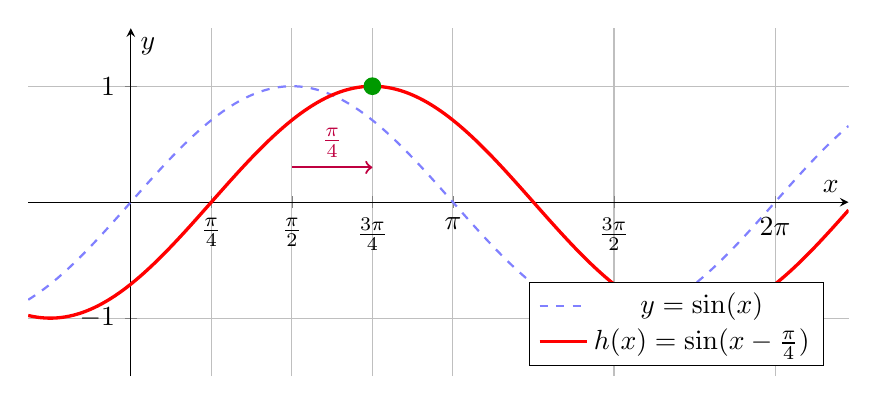
\begin{tikzpicture}
\begin{axis}[
    width=12cm,
    height=6cm,
    axis lines=middle,
    xlabel={$x$},
    ylabel={$y$},
    domain=-1:7,
    samples=200,
    ymin=-1.5,
    ymax=1.5,
    xmin=-1,
    xmax=7,
    xtick={0,0.7854,1.5708,2.3562,3.1416,4.7124,6.2832},
    xticklabels={$0$,$\frac{\pi}{4}$,$\frac{\pi}{2}$,$\frac{3\pi}{4}$,$\pi$,$\frac{3\pi}{2}$,$2\pi$},
    ytick={-1,0,1},
    grid=major,
    legend pos=south east,
]
    % Función original
    \addplot[blue!50,dashed,thick] {sin(deg(x))};
    \addlegendentry{$y = \sin(x)$}

    % Función transformada
    \addplot[red,very thick] {sin(deg(x - pi/4))};
    \addlegendentry{$h(x) = \sin(x - \frac{\pi}{4})$}

    % Marcar el punto máximo
    \addplot[only marks,mark=*,mark size=3pt,color=green!60!black] coordinates {(2.3562,1)};

    % Flecha indicando el desfase
    \draw[->,thick,purple] (axis cs:1.5708,0.3) -- (axis cs:2.3562,0.3) node[midway,above] {$\frac{\pi}{4}$};
\end{axis}
\end{tikzpicture}
\end{center}

\textbf{Verificación:}
\[
h\left(\frac{3\pi}{4}\right) = \sin\left(\frac{3\pi}{4} - \frac{\pi}{4}\right) = \sin\left(\frac{\pi}{2}\right) = 1 \quad \checkmark
\]
\end{solucion}

\begin{solucion}[title=Solucion Ejercicio 4]
\textbf{Dada:} $k(x) = -2\cos(x) + 1$

\textbf{Parte a):} Transformaciones aplicadas

Partiendo de $y = \cos(x)$, se aplican las siguientes transformaciones:

\begin{enumerate}
    \item \textbf{Multiplicación por 2:} Estiramiento vertical con factor 2 → $2\cos(x)$
    \item \textbf{Multiplicación por -1:} Reflexión sobre el eje $x$ → $-2\cos(x)$
    \item \textbf{Suma de 1:} Desplazamiento vertical hacia arriba 1 unidad → $-2\cos(x) + 1$
\end{enumerate}

\textbf{Respuesta a):} $\boxed{\text{Estiramiento vertical (factor 2), reflexión sobre el eje } x, \text{ desfase vertical (+1)}}$

\textbf{Parte b):} Amplitud

La amplitud es el valor absoluto del coeficiente que multiplica a $\cos(x)$:
\[
\text{Amplitud} = |-2| = 2
\]

\textbf{Respuesta b):} $\boxed{\text{Amplitud} = 2}$

\textbf{Parte c):} Valores máximo y mínimo

El coseno básico oscila entre -1 y 1. Aplicamos las transformaciones paso a paso:

\textbf{Paso 1:} $\cos(x) \in [-1, 1]$

\textbf{Paso 2:} Multiplicar por -2 invierte y estira: $-2\cos(x) \in [-2, 2]$
\begin{itemize}
    \item Cuando $\cos(x) = 1$: $-2(1) = -2$
    \item Cuando $\cos(x) = -1$: $-2(-1) = 2$
\end{itemize}

\textbf{Paso 3:} Sumar 1 desplaza hacia arriba: $-2\cos(x) + 1 \in [-2+1, 2+1] = [-1, 3]$

Por lo tanto:
\begin{itemize}
    \item Valor máximo: $k_{\max} = 3$ (cuando $\cos(x) = -1$)
    \item Valor mínimo: $k_{\min} = -1$ (cuando $\cos(x) = 1$)
\end{itemize}

\textbf{Respuesta c):} $\boxed{\text{Máximo} = 3, \quad \text{Mínimo} = -1}$

\textbf{Parte d):} Eje de simetría (línea central)

El eje de simetría es la línea que pasa por el punto medio entre el máximo y el mínimo:
\[
\text{Eje de simetría: } y = \frac{k_{\max} + k_{\min}}{2} = \frac{3 + (-1)}{2} = \frac{2}{2} = 1
\]

Otra forma: el eje de simetría está dado por el desfase vertical, que es $D = 1$.

\textbf{Respuesta d):} $\boxed{y = 1}$

\textbf{Gráfica:}

\begin{center}
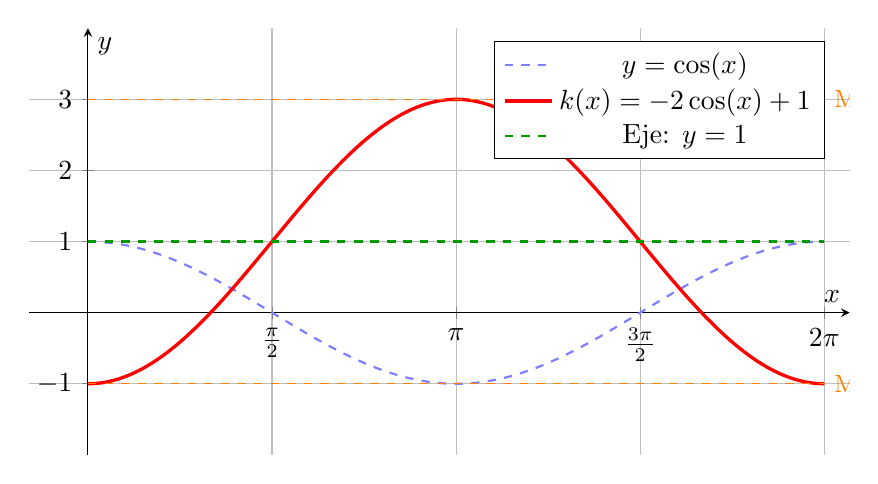
\begin{tikzpicture}
\begin{axis}[
    width=12cm,
    height=7cm,
    axis lines=middle,
    xlabel={$x$},
    ylabel={$y$},
    domain=0:2*pi,
    samples=200,
    ymin=-2,
    ymax=4,
    xmin=-0.5,
    xmax=6.5,
    xtick={0,1.5708,3.1416,4.7124,6.2832},
    xticklabels={$0$,$\frac{\pi}{2}$,$\pi$,$\frac{3\pi}{2}$,$2\pi$},
    ytick={-1,0,1,2,3},
    grid=major,
    legend pos=north east,
]
    % Función original
    \addplot[blue!50,dashed,thick] {cos(deg(x))};
    \addlegendentry{$y = \cos(x)$}

    % Función transformada
    \addplot[red,very thick] {-2*cos(deg(x)) + 1};
    \addlegendentry{$k(x) = -2\cos(x) + 1$}

    % Eje de simetría
    \addplot[green!60!black,dashed,thick] {1};
    \addlegendentry{Eje: $y = 1$}

    % Líneas de máximo y mínimo
    \draw[orange,dashed] (axis cs:0,3) -- (axis cs:6.2832,3) node[right,font=\small] {Máximo = 3};
    \draw[orange,dashed] (axis cs:0,-1) -- (axis cs:6.2832,-1) node[right,font=\small] {Mínimo = -1};
\end{axis}
\end{tikzpicture}
\end{center}

\textbf{Verificación:}
\begin{itemize}
    \item En $x = 0$: $k(0) = -2\cos(0) + 1 = -2(1) + 1 = -1$ \checkmark (mínimo)
    \item En $x = \pi$: $k(\pi) = -2\cos(\pi) + 1 = -2(-1) + 1 = 3$ \checkmark (máximo)
\end{itemize}
\end{solucion}

\begin{solucion}[title=Solucion Ejercicio 5]
\textbf{Dada:} $f(x) = 2\sin(3x)$ en $[0, 2\pi]$

\textbf{Parte a):} Amplitud

\[
\text{Amplitud} = |A| = |2| = 2
\]

\textbf{Respuesta a):} $\boxed{\text{Amplitud} = 2}$

\textbf{Parte b):} Período

\[
\text{Período} = \frac{2\pi}{B} = \frac{2\pi}{3}
\]

\textbf{Respuesta b):} $\boxed{\text{Período} = \frac{2\pi}{3}}$

\textbf{Parte c):} Número de ciclos en $[0, 2\pi]$

\[
\text{Número de ciclos} = \frac{\text{Longitud del intervalo}}{\text{Período}} = \frac{2\pi}{2\pi/3} = \frac{2\pi \cdot 3}{2\pi} = 3
\]

\textbf{Respuesta c):} $\boxed{3 \text{ ciclos completos}}$

\textbf{Parte d):} Primeros tres máximos

La función seno alcanza su máximo cuando el argumento es $\frac{\pi}{2} + 2\pi k$:
\[
3x = \frac{\pi}{2} + 2\pi k
\]
\[
x = \frac{\pi}{6} + \frac{2\pi k}{3}
\]

Para los primeros tres máximos ($k = 0, 1, 2$):

\textbf{Primer máximo} ($k = 0$):
\[
x_1 = \frac{\pi}{6}, \quad f\left(\frac{\pi}{6}\right) = 2\sin\left(3 \cdot \frac{\pi}{6}\right) = 2\sin\left(\frac{\pi}{2}\right) = 2
\]
Punto: $\left(\frac{\pi}{6}, 2\right)$

\textbf{Segundo máximo} ($k = 1$):
\[
x_2 = \frac{\pi}{6} + \frac{2\pi}{3} = \frac{\pi}{6} + \frac{4\pi}{6} = \frac{5\pi}{6}
\]
Punto: $\left(\frac{5\pi}{6}, 2\right)$

\textbf{Tercer máximo} ($k = 2$):
\[
x_3 = \frac{\pi}{6} + \frac{4\pi}{3} = \frac{\pi}{6} + \frac{8\pi}{6} = \frac{9\pi}{6} = \frac{3\pi}{2}
\]
Punto: $\left(\frac{3\pi}{2}, 2\right)$

\textbf{Respuesta d):} $\boxed{\left(\frac{\pi}{6}, 2\right), \quad \left(\frac{5\pi}{6}, 2\right), \quad \left(\frac{3\pi}{2}, 2\right)}$

\textbf{Gráfica:}

\begin{center}
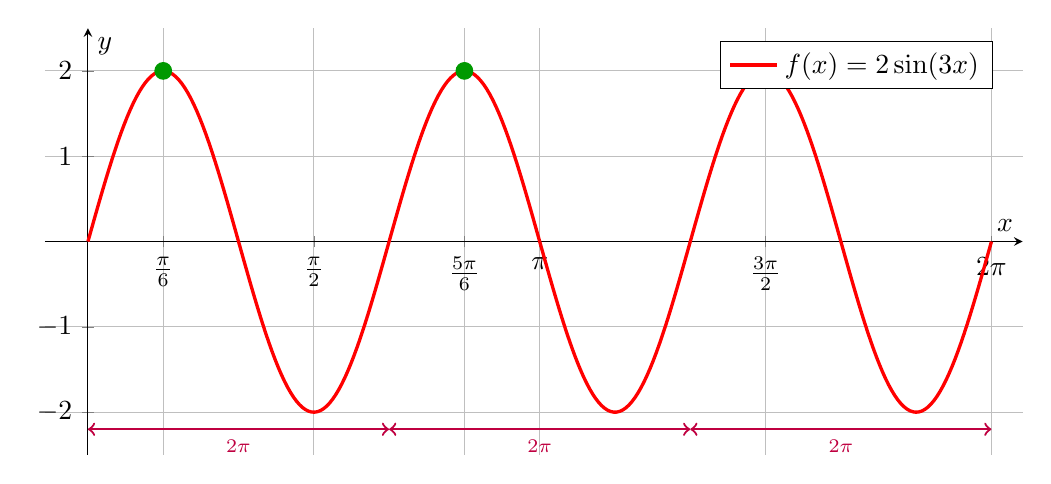
\begin{tikzpicture}
\begin{axis}[
    width=14cm,
    height=7cm,
    axis lines=middle,
    xlabel={$x$},
    ylabel={$y$},
    domain=0:2*pi,
    samples=300,
    ymin=-2.5,
    ymax=2.5,
    xmin=-0.3,
    xmax=6.5,
    xtick={0,0.5236,1.5708,2.618,3.1416,4.7124,6.2832},
    xticklabels={$0$,$\frac{\pi}{6}$,$\frac{\pi}{2}$,$\frac{5\pi}{6}$,$\pi$,$\frac{3\pi}{2}$,$2\pi$},
    ytick={-2,-1,0,1,2},
    grid=major,
    legend pos=north east,
]
    % Función transformada
    \addplot[red,very thick] {2*sin(3*deg(x))};
    \addlegendentry{$f(x) = 2\sin(3x)$}

    % Marcar los tres primeros máximos
    \addplot[only marks,mark=*,mark size=3pt,color=green!60!black] coordinates {(0.5236,2) (2.618,2) (4.7124,2)};

    % Indicar los períodos
    \draw[<->,thick,purple] (axis cs:0,-2.2) -- (axis cs:2.0944,-2.2) node[midway,below] {$\frac{2\pi}{3}$};
    \draw[<->,thick,purple] (axis cs:2.0944,-2.2) -- (axis cs:4.1888,-2.2) node[midway,below] {$\frac{2\pi}{3}$};
    \draw[<->,thick,purple] (axis cs:4.1888,-2.2) -- (axis cs:6.2832,-2.2) node[midway,below] {$\frac{2\pi}{3}$};
\end{axis}
\end{tikzpicture}
\end{center}

\textbf{Observación:} La función oscila 3 veces más rápido que $\sin(x)$ debido al factor $B = 3$.
\end{solucion}

\begin{solucion}[title=Solucion Ejercicio 6]
\textbf{Dada:} $m(x) = \cos(x + \frac{\pi}{3}) - 2$

\textbf{Parte a):} Desfase horizontal y dirección

La función tiene la forma $\cos(x + C)$ donde $C = \frac{\pi}{3}$.

Como es una suma (signo positivo), el desfase es hacia la \textbf{izquierda}.

Magnitud del desfase: $\frac{\pi}{3}$ radianes.

\textbf{Respuesta a):} $\boxed{\text{Desfase de } \frac{\pi}{3} \text{ hacia la izquierda}}$

\textbf{Parte b):} Desfase vertical y dirección

El término $-2$ al final representa un desplazamiento vertical de 2 unidades hacia \textbf{abajo}.

\textbf{Respuesta b):} $\boxed{\text{Desfase de 2 unidades hacia abajo}}$

\textbf{Parte c):} Rango

El coseno básico tiene rango $[-1, 1]$.

Aplicando las transformaciones:
\[
\cos(x + \frac{\pi}{3}) \in [-1, 1]
\]
\[
\cos(x + \frac{\pi}{3}) - 2 \in [-1-2, 1-2] = [-3, -1]
\]

\textbf{Respuesta c):} $\boxed{\text{Rango} = [-3, -1]}$

\textbf{Parte d):} Gráfica en $[-\pi, 2\pi]$

\begin{center}
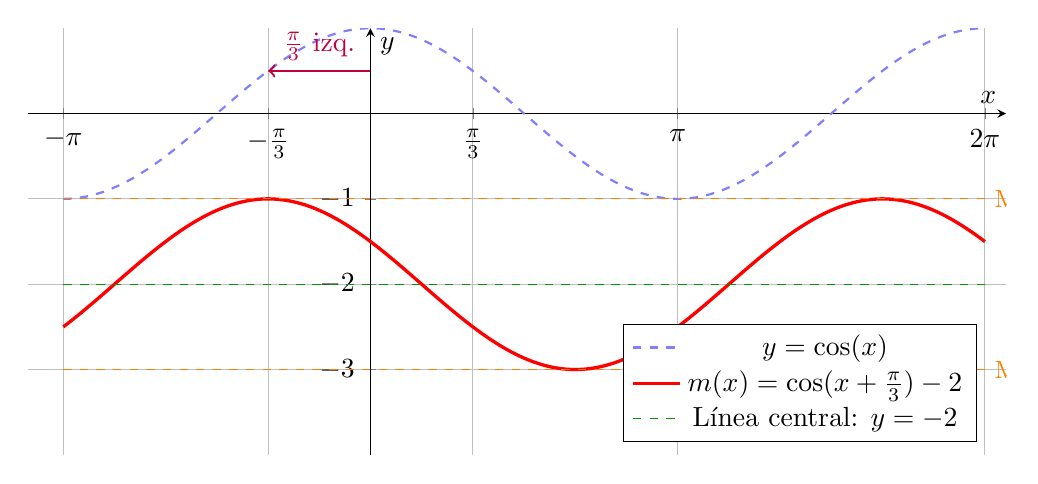
\begin{tikzpicture}
\begin{axis}[
    width=14cm,
    height=7cm,
    axis lines=middle,
    xlabel={$x$},
    ylabel={$y$},
    domain=-pi:2*pi,
    samples=300,
    ymin=-4,
    ymax=1,
    xmin=-3.5,
    xmax=6.5,
    xtick={-3.1416,-1.0472,0,1.0472,3.1416,6.2832},
    xticklabels={$-\pi$,$-\frac{\pi}{3}$,$0$,$\frac{\pi}{3}$,$\pi$,$2\pi$},
    ytick={-3,-2,-1,0},
    grid=major,
    legend pos=south east,
]
    % Función original
    \addplot[blue!50,dashed,thick] {cos(deg(x))};
    \addlegendentry{$y = \cos(x)$}

    % Función transformada
    \addplot[red,very thick] {cos(deg(x + pi/3)) - 2};
    \addlegendentry{$m(x) = \cos(x + \frac{\pi}{3}) - 2$}

    % Línea central
    \addplot[green!60!black,dashed] {-2};
    \addlegendentry{Línea central: $y = -2$}

    % Rango
    \draw[orange,dashed] (axis cs:-3.1416,-3) -- (axis cs:6.2832,-3) node[right,font=\small] {Mínimo = -3};
    \draw[orange,dashed] (axis cs:-3.1416,-1) -- (axis cs:6.2832,-1) node[right,font=\small] {Máximo = -1};

    % Flecha mostrando desfase horizontal
    \draw[->,thick,purple] (axis cs:0,0.5) -- (axis cs:-1.0472,0.5) node[midway,above] {$\frac{\pi}{3}$ izq.};
\end{axis}
\end{tikzpicture}
\end{center}

\textbf{Puntos clave:}
\begin{itemize}
    \item Máximo en $x = -\frac{\pi}{3}$: $m(-\frac{\pi}{3}) = \cos(0) - 2 = 1 - 2 = -1$ \checkmark
    \item Mínimo en $x = \frac{2\pi}{3}$: $m(\frac{2\pi}{3}) = \cos(\pi) - 2 = -1 - 2 = -3$ \checkmark
    \item Intercepto en $y$: $m(0) = \cos(\frac{\pi}{3}) - 2 = \frac{1}{2} - 2 = -\frac{3}{2}$ \checkmark
\end{itemize}
\end{solucion}

\begin{solucion}[title=Solucion Ejercicio 7]
\textbf{Dada:} $p(x) = 4\sin(\frac{1}{2}x - \pi) + 3$

Primero, reescribimos la función en la forma estándar:
\[
p(x) = A\sin(B(x - C)) + D
\]

Factorizando el $\frac{1}{2}$ del argumento:
\[
p(x) = 4\sin\left(\frac{1}{2}\left(x - 2\pi\right)\right) + 3
\]

Aquí: $A = 4$, $B = \frac{1}{2}$, $C = 2\pi$, $D = 3$

\textbf{Parte a):} Amplitud

\[
\text{Amplitud} = |A| = |4| = 4
\]

\textbf{Respuesta a):} $\boxed{\text{Amplitud} = 4}$

\textbf{Parte b):} Período

\[
\text{Período} = \frac{2\pi}{B} = \frac{2\pi}{1/2} = 2\pi \cdot 2 = 4\pi
\]

\textbf{Respuesta b):} $\boxed{\text{Período} = 4\pi}$

\textbf{Parte c):} Desfase horizontal

De la forma factorizada $\sin\left(\frac{1}{2}(x - 2\pi)\right)$, vemos que:
\[
C = 2\pi
\]

Esto significa un desfase de $2\pi$ radianes hacia la \textbf{derecha}.

\textbf{Respuesta c):} $\boxed{\text{Desfase horizontal} = 2\pi \text{ hacia la derecha}}$

\textbf{Parte d):} Desfase vertical

\[
D = 3
\]

Esto representa un desplazamiento de 3 unidades hacia \textbf{arriba}.

\textbf{Respuesta d):} $\boxed{\text{Desfase vertical} = 3 \text{ hacia arriba}}$

\textbf{Parte e):} Rango

La amplitud es 4 y el eje central está en $y = 3$, por lo tanto:
\begin{align*}
\text{Mínimo} &= D - A = 3 - 4 = -1 \\
\text{Máximo} &= D + A = 3 + 4 = 7
\end{align*}

\textbf{Respuesta e):} $\boxed{\text{Rango} = [-1, 7]}$

\textbf{Gráfica:}

\begin{center}
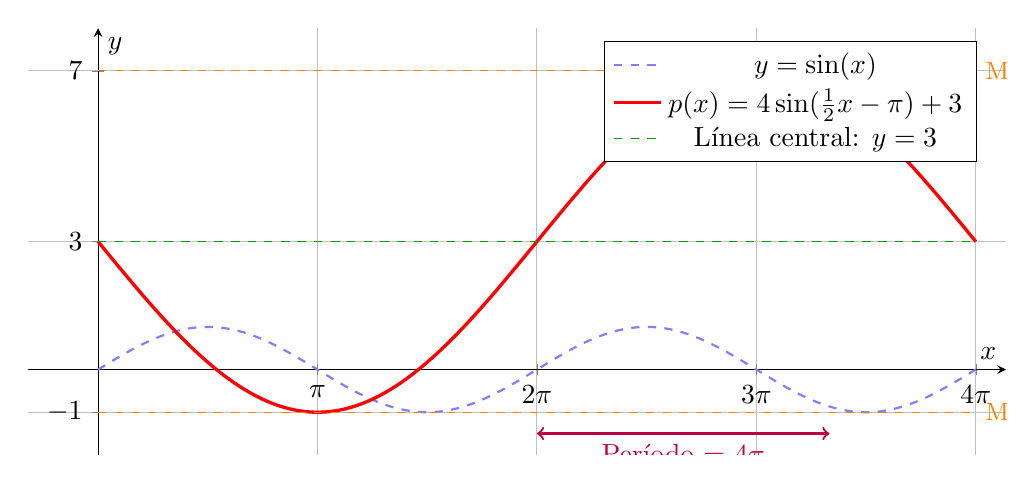
\begin{tikzpicture}
\begin{axis}[
    width=14cm,
    height=7cm,
    axis lines=middle,
    xlabel={$x$},
    ylabel={$y$},
    domain=0:4*pi,
    samples=300,
    ymin=-2,
    ymax=8,
    xmin=-1,
    xmax=13,
    xtick={0,3.1416,6.2832,9.4248,12.5664},
    xticklabels={$0$,$\pi$,$2\pi$,$3\pi$,$4\pi$},
    ytick={-1,0,3,7},
    grid=major,
    legend pos=north east,
]
    % Función original
    \addplot[blue!50,dashed,thick,domain=0:12.5664] {sin(deg(x))};
    \addlegendentry{$y = \sin(x)$}

    % Función transformada
    \addplot[red,very thick] {4*sin(deg(0.5*x - pi)) + 3};
    \addlegendentry{$p(x) = 4\sin(\frac{1}{2}x - \pi) + 3$}

    % Línea central
    \addplot[green!60!black,dashed] {3};
    \addlegendentry{Línea central: $y = 3$}

    % Líneas de rango
    \draw[orange,dashed] (axis cs:0,7) -- (axis cs:12.5664,7) node[right,font=\small] {Máx = 7};
    \draw[orange,dashed] (axis cs:0,-1) -- (axis cs:12.5664,-1) node[right,font=\small] {Mín = -1};

    % Período
    \draw[<->,thick,purple] (axis cs:6.2832,-1.5) -- (axis cs:10.472,-1.5) node[midway,below] {Período = $4\pi$};
\end{axis}
\end{tikzpicture}
\end{center}

\textbf{Análisis completo:}

\begin{itemize}
    \item La amplitud de 4 hace que la función oscile 4 unidades arriba y abajo del eje central
    \item El período de $4\pi$ significa que la función completa un ciclo cada $4\pi$ unidades (mucho más lento que $\sin(x)$)
    \item El desfase de $2\pi$ a la derecha mueve toda la gráfica hacia la derecha
    \item El desfase vertical de 3 eleva toda la función 3 unidades
\end{itemize}

\textbf{Verificación del primer máximo:}

El máximo ocurre cuando $\frac{1}{2}x - \pi = \frac{\pi}{2}$:
\[
\frac{1}{2}x = \frac{\pi}{2} + \pi = \frac{3\pi}{2}
\]
\[
x = 3\pi
\]

Verificamos:
\[
p(3\pi) = 4\sin\left(\frac{3\pi}{2} - \pi\right) + 3 = 4\sin\left(\frac{\pi}{2}\right) + 3 = 4(1) + 3 = 7 \quad \checkmark
\]
\end{solucion}

\begin{solucion}[title=Solucion Ejercicio 8]
\textbf{Dada:} $h(t) = 5\cos\left(\frac{\pi}{6}t\right) + 8$

donde $h$ está en metros y $t$ es el tiempo en horas después de medianoche.

\textbf{Identificación de parámetros:}
\begin{itemize}
    \item Amplitud: $A = 5$ metros
    \item Frecuencia angular: $B = \frac{\pi}{6}$
    \item Desfase vertical: $D = 8$ metros (altura media)
\end{itemize}

\textbf{Parte a):} Altura máxima

La altura máxima es:
\[
h_{\max} = D + A = 8 + 5 = 13 \text{ metros}
\]

\textbf{Respuesta a):} $\boxed{13 \text{ metros}}$

\textbf{Parte b):} Altura mínima

La altura mínima es:
\[
h_{\min} = D - A = 8 - 5 = 3 \text{ metros}
\]

\textbf{Respuesta b):} $\boxed{3 \text{ metros}}$

\textbf{Parte c):} Período de la marea

\[
\text{Período} = \frac{2\pi}{B} = \frac{2\pi}{\pi/6} = 2\pi \cdot \frac{6}{\pi} = 12 \text{ horas}
\]

Esto tiene sentido físicamente: las mareas siguen un ciclo de aproximadamente 12 horas.

\textbf{Respuesta c):} $\boxed{12 \text{ horas}}$

\textbf{Parte d):} Primera marea alta después de medianoche

La función coseno alcanza su máximo cuando el argumento es 0 (o múltiplos de $2\pi$):
\[
\frac{\pi}{6}t = 0
\]
\[
t = 0
\]

Esto significa que la primera marea alta ocurre exactamente a \textbf{medianoche} (00:00 horas).

La siguiente marea alta ocurre cuando:
\[
\frac{\pi}{6}t = 2\pi
\]
\[
t = 12 \text{ horas (mediodía)}
\]

\textbf{Respuesta d):} $\boxed{t = 0 \text{ horas (medianoche, 12:00 AM)}}$

\textbf{Parte e):} Altura a las 9:00 AM

A las 9:00 AM, han pasado $t = 9$ horas desde medianoche:
\begin{align*}
h(9) &= 5\cos\left(\frac{\pi}{6} \cdot 9\right) + 8 \\
&= 5\cos\left(\frac{9\pi}{6}\right) + 8 \\
&= 5\cos\left(\frac{3\pi}{2}\right) + 8 \\
&= 5(0) + 8 \\
&= 8 \text{ metros}
\end{align*}

A las 9:00 AM, la marea está exactamente en su altura media.

\textbf{Respuesta e):} $\boxed{8 \text{ metros}}$

\textbf{Gráfica de la marea durante 24 horas:}

\begin{center}
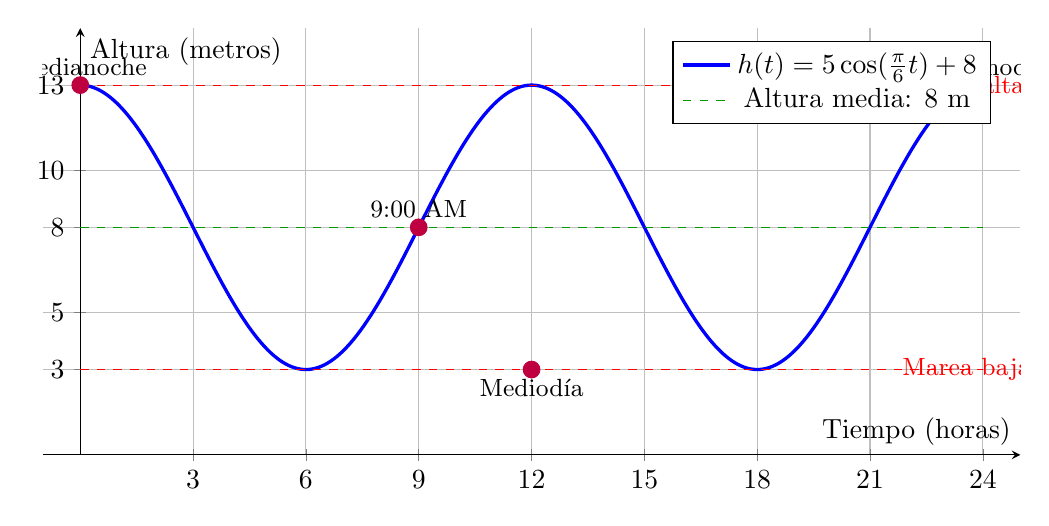
\begin{tikzpicture}
\begin{axis}[
    width=14cm,
    height=7cm,
    axis lines=middle,
    xlabel={Tiempo (horas)},
    ylabel={Altura (metros)},
    domain=0:24,
    samples=300,
    ymin=0,
    ymax=15,
    xmin=-1,
    xmax=25,
    xtick={0,3,6,9,12,15,18,21,24},
    ytick={0,3,5,8,10,13},
    grid=major,
    legend pos=north east,
]
    % Función de la marea
    \addplot[blue,very thick] {5*cos(deg(pi*x/6)) + 8};
    \addlegendentry{$h(t) = 5\cos(\frac{\pi}{6}t) + 8$}

    % Altura media
    \addplot[green!60!black,dashed] {8};
    \addlegendentry{Altura media: 8 m}

    % Máximos y mínimos
    \addplot[red,dashed] {13} node[right,pos=0.9,font=\small] {Marea alta: 13 m};
    \addplot[red,dashed] {3} node[right,pos=0.9,font=\small] {Marea baja: 3 m};

    % Marcar puntos importantes
    \addplot[only marks,mark=*,mark size=3pt,color=purple] coordinates {(0,13) (9,8) (12,3) (24,13)};

    % Etiquetas de puntos
    \node[above] at (axis cs:0,13) {\small Medianoche};
    \node[above] at (axis cs:9,8) {\small 9:00 AM};
    \node[below] at (axis cs:12,3) {\small Mediodía};
    \node[above] at (axis cs:24,13) {\small Medianoche};
\end{axis}
\end{tikzpicture}
\end{center}

\textbf{Interpretación física:}

\begin{itemize}
    \item A medianoche (00:00), la marea está en su punto más alto: 13 metros
    \item La marea baja gradualmente durante la mañana
    \item A las 9:00 AM, está en su altura media: 8 metros
    \item Al mediodía (12:00), alcanza su punto más bajo: 3 metros
    \item Luego comienza a subir nuevamente
    \item A las 6:00 PM, vuelve a la altura media
    \item A la medianoche siguiente, vuelve a estar alta
\end{itemize}

\textbf{Tabla de valores clave:}

\begin{center}
\begin{tabular}{|c|c|c|}
\hline
\textbf{Hora} & \textbf{$t$ (horas)} & \textbf{Altura (m)} \\
\hline
Medianoche & 0 & 13 (máx) \\
3:00 AM & 3 & 10.5 \\
6:00 AM & 6 & 8 (media) \\
9:00 AM & 9 & 5.5 \\
Mediodía & 12 & 3 (mín) \\
3:00 PM & 15 & 5.5 \\
6:00 PM & 18 & 8 (media) \\
9:00 PM & 21 & 10.5 \\
Medianoche & 24 & 13 (máx) \\
\hline
\end{tabular}
\end{center}

\textbf{Conclusión:} Este modelo matemático representa de manera muy realista el comportamiento de las mareas, que son causadas principalmente por la atracción gravitacional de la Luna y el Sol.
\end{solucion}
